\documentclass[9pt]{jsarticle}
\usepackage[dvipdfmx,hiresbb]{graphicx}
\usepackage{amsmath,amssymb}
\usepackage{float}
\usepackage{bm}
\usepackage{wrapfig}
\usepackage{booktabs}
\usepackage{subcaption}
\usepackage{braket}
\usepackage[english]{babel}
\usepackage{ascmac}
%\usepackage[top=2cm, bottom=5mm, left=5mm, right=1cm]{geometry}
\usepackage{tikz}
\usepackage{subcaption}
\usepackage{multirow}
\usepackage{amssymb}
\title{Description about conservative horizontal momentum diffusion scheme and tensorial stress option in LFRic}
\author{Shusuke Nishimoto}
\date{\hfill}
\begin{document}
\maketitle

\section{Equation of diffusion scheme}

In LFRic's Smagorinsky scheme and blending boundary layer scheme \cite{boutle14}, subgrid turbulent mixing of momentum is calculated by the following equation:
\begin{equation}
  \frac{\partial u_i}{\partial t} = -\frac{1}{\rho} \frac{\partial F^{u_i, x_j} }{\partial x_j} \quad\quad \left( F^{u_i, x_j} = -\rho\nu \frac{\partial u_i}{\partial x_j} \right),
  \label{eq:base}
\end{equation}
where $\rho$ and $\nu$ are density and mixing coefficient, respectively. $u_i$ and $x_i$ are 3-dimensional cartesian velocity and coordinate following Einstein's notation rule.
Imcompressive formulation is adopted, so density is ignored in the horizontal diffusion, so each $F^{u_i, x_j}$ is represented as follows:
\begin{equation*}
  F^{ux} = -\nu \frac{\partial u}{\partial x}, \quad
  F^{uy} = -\nu \frac{\partial u}{\partial y}, \quad
  F^{uz} = \textcolor{red}{-\nu \frac{\partial u}{\partial z}},
\end{equation*}
\begin{equation*}
  F^{vx} = -\nu \frac{\partial v}{\partial x}, \quad
  F^{vy} = -\nu \frac{\partial v}{\partial y}, \quad
  F^{vz} = \textcolor{red}{-\nu \frac{\partial v}{\partial z}},
\end{equation*}
\begin{equation*}
  F^{wx} = -\nu \frac{\partial w}{\partial x}, \quad
  F^{wy} = -\nu \frac{\partial w}{\partial y}, \quad
  F^{wz} = \textcolor{red}{-\nu \frac{\partial w}{\partial z}},
\end{equation*}
where $x, y, z, u, v$ and $w$ are 3-dimensional coordinate and wind components, respectively.
Since, red colored terms are calculated not in the diffusion scheme but in the boundary layer scheme, we ignore them in the following explanation.
The equations for $u, v, w$ are as follows:
\begin{equation}
  \frac{\partial u}{\partial t} = -\frac{\partial F^{ux}}{\partial x} - \frac{\partial F^{uy}}{\partial y},
  \label{eq:baseu}
\end{equation}
\begin{equation}
  \frac{\partial v}{\partial t} = -\frac{\partial F^{vx}}{\partial x} - \frac{\partial F^{vy}}{\partial y},
  \label{eq:basev}
\end{equation}
\begin{equation}
  \frac{\partial w}{\partial t} = -\frac{\partial F^{wx}}{\partial x} - \frac{\partial F^{wy}}{\partial y}.
  \label{eq:basew}
\end{equation}

\section{Conservative horizontal diffusion}

Here, we will explain how to calculate (\ref{eq:baseu}), (\ref{eq:basev}) and (\ref{eq:basew}).
In the following, as shown in Figure\ref{fig:grid_def}, locations that are half-grid shifted relative to grid numbers $i, j$ and $k$ will be represented as $i+\frac{1}{2}, j+\frac{1}{2}$ and $k+\frac{1}{2}$, respectively.

In LFRic, $u, v$ and $w$ are placed on the face of each cell as shown in Figure\ref{fig:wind_def_point}.

\begin{figure}[h]
  \centering
  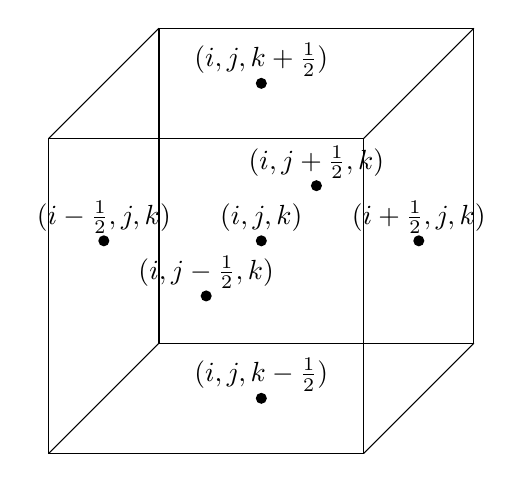
\begin{tikzpicture}
    \draw (0,0) rectangle (4,4);
    \draw (1.4,1.4) rectangle (5.4,5.4); 
    \draw (0,0) -- (1.4,1.4);
    \draw (0,4) -- (1.4,5.4);
    \draw (4,0) -- (5.4,1.4);
    \draw (4,4) -- (5.4,5.4);
    \fill (2.7,2.7) circle (2pt);
    \node at (2.7,3.0) {$(i,j,k)$};
    \fill (0.7,2.7) circle (2pt);
    \node at (0.7,3.0) {$(i-\frac{1}{2},j,k)$};
    \fill (4.7,2.7) circle (2pt);
    \node at (4.7,3.0) {$(i+\frac{1}{2},j,k)$};
    \fill (2.0,2.0) circle (2pt);
    \node at (2.0,2.3) {$(i,j-\frac{1}{2},k)$};
    \fill (3.4,3.4) circle (2pt);
    \node at (3.4,3.7) {$(i,j+\frac{1}{2},k)$};
    \fill (2.7,0.7) circle (2pt);
    \node at (2.7,1.0) {$(i,j,k-\frac{1}{2})$};
    \fill (2.7,4.7) circle (2pt);
    \node at (2.7,5.0) {$(i,j,k+\frac{1}{2})$};
  \end{tikzpicture}
  \hspace{20pt}
  \begin{tikzpicture}
    \draw[->] (-0.5,0) -- (2.0,0.0) node[right] {$x$};
    \draw[->] (0,-0.5) -- (0.0,2.0) node[right] {$z$};
    \draw[->] (-0.3,-0.3) -- (1.4,1.4) node[right] {$y$};
  \end{tikzpicture}
  \caption{Notation of grid number. Cube indecates $(i,j,k)$th cell.}
  \label{fig:grid_def}
\end{figure}
\begin{figure}[h]
  \vspace{-15pt}
  \centering
  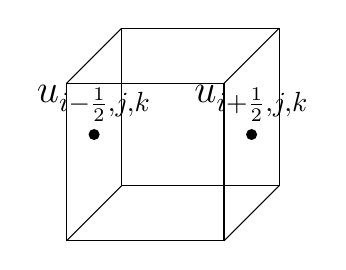
\begin{tikzpicture}
    \draw (0,0) rectangle (2,2);
    \draw (0.7,0.7) rectangle (2.7,2.7); 
    \draw (0,0) -- (0.7,0.7);
    \draw (0,2) -- (0.7,2.7);
    \draw (2,0) -- (2.7,0.7);
    \draw (2,2) -- (2.7,2.7);
    \fill (0.35,1.35) circle (2pt);
    \fill (2.35,1.35) circle (2pt);
    \node at (2.35,1.75) {\Large $u_{i+\frac{1}{2},j,k}$};
    \node at (0.35,1.75) {\Large $u_{i-\frac{1}{2},j,k}$};
 \end{tikzpicture}
 \hspace{20pt} 
 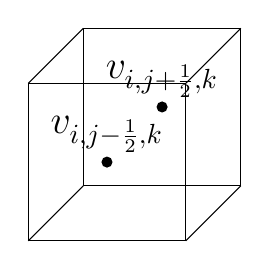
\begin{tikzpicture}
    \draw (0,0) rectangle (2,2);
    \draw (0.7,0.7) rectangle (2.7,2.7); 
    \draw (0,0) -- (0.7,0.7);
    \draw (0,2) -- (0.7,2.7);
    \draw (2,0) -- (2.7,0.7);
    \draw (2,2) -- (2.7,2.7);
    \fill (1,1) circle (2pt);
    \fill (1.7,1.7) circle (2pt);
    \node at (1.7,2.05) {\Large $v_{i,j+\frac{1}{2},k}$};
    \node at (1,1.35) {\Large $v_{i,j-\frac{1}{2},k}$};
 \end{tikzpicture}
 \hspace{20pt}
 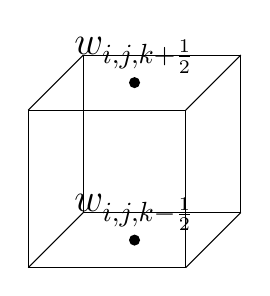
\begin{tikzpicture}
    \draw (0,0) rectangle (2,2);
    \draw (0.7,0.7) rectangle (2.7,2.7); 
    \draw (0,0) -- (0.7,0.7);
    \draw (0,2) -- (0.7,2.7);
    \draw (2,0) -- (2.7,0.7);
    \draw (2,2) -- (2.7,2.7);
    \fill (1.35,2.35) circle (2pt);
    \fill (1.35,0.35) circle (2pt);
    \node at (1.35,2.7) {\Large $w_{i,j,k+\frac{1}{2}}$};
    \node at (1.35,0.7) {\Large $w_{i,j,k-\frac{1}{2}}$};
 \end{tikzpicture}
 \caption{Definition point of each velocity on the face of $(i,j,k)$th cell.}
 \label{fig:wind_def_point}
\end{figure}

\newpage
\vspace{-10pt}
In the calculation of (\ref{eq:baseu}) for $u_{i+\frac{1}{2},j,k}$, we assume a volume $V_{i+\frac{1}{2},j,k}$ surrounding $u_{i+\frac{1}{2},j,k}$.
$\nu$ is linearly interpolated to the face of $V_{i+\frac{1}{2},j,k}$, and wind shears are also evaluated at the same locations.
$F^{ux}$ and $F^{uy}$ are calculated on the face of $V_{i+\frac{1}{2},j,k}$ by multiplying them as depected in Figure\ref{fig:def_point_uflux}.
Increment of $u_{i+\frac{1}{2},j,k}$ is calculated as:
\vspace{-5pt}
\begin{equation}
  \Delta u_{i+\frac{1}{2},j,k} = - \frac{
        \left( F^{ux}_{i+1,j,k} A^{x}_{i+1,j,k} - F^{ux}_{i,j,k} A^{x}_{i,j,k} \right)
      + \left( F^{uy}_{i,j+\frac{1}{2},k} A^{y}_{i,j+\frac{1}{2},k} - F^{uy}_{i,j-\frac{1}{2},k} A^{y}_{i,j-\frac{1}{2},k} \right)
                                        }{ V_{i+\frac{1}{2},j,k} } \Delta t,
  \label{eq:disc_diff_u}
\end{equation}
where $A^{x}$ and $A^{y}$ are the area of faces on which $F^{ux}$ and $F^{uy}$ are placed, respectively.
Please see Figure\ref{fig:def_point_uflux} for placement of each term in (\ref{eq:disc_diff_u}).
Since adjacent cells share the same $F^{ux} A^{x}$ and $F^{uy} A^{y}$ at their boundary, the increment of total volume-weighed $u$ is cancelled out by summing up (\ref{eq:disc_diff_u}) and ignoring the effect of lateral boundary condition:
\vspace{-5pt}
\begin{equation}
  \Delta \left( \sum_{i,j,k} V_{i+\frac{1}{2},j,k} u_{i+\frac{1}{2},j,k} \right) = \sum_{i,j,k} V_{i+\frac{1}{2},j,k} \Delta u_{i+\frac{1}{2},j,k} = 0,
\end{equation}
which means (\ref{eq:disc_diff_u}) conserves volume-weighed total $u$.

\vspace{-10pt}
\begin{figure}[h]
\centering
\begin{subfigure}{0.3\linewidth}
  \centering
  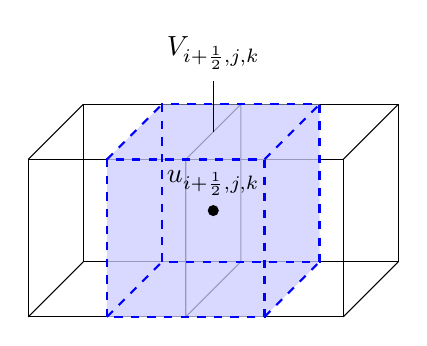
\begin{tikzpicture}
    \draw (0,0) rectangle (4,2);
    \draw (0.7,0.7) rectangle (4.7,2.7);
  
    \draw (0,0) -- (0.7,0.7);
    \draw (4,0) -- (4.7,0.7);
    \draw (0,2) -- (0.7,2.7);
    \draw (4,2) -- (4.7,2.7);
  
    \draw (2.0,0.0) -- (2.7,0.7) -- (2.7,2.7) -- (2.0,2.0) -- cycle;
 
    \filldraw[fill=blue!20, draw=none, opacity=0.75] (1.0,0.0) -- (3.0,0.0) -- (3.7,0.7) -- (3.7,2.7) -- (1.7,2.7) -- (1.0,2.0) -- cycle;
    \draw[blue, thick, dashed] (1.0,0.0) rectangle (3.0,2.0);
    \draw[blue, thick, dashed] (1.7,0.7) rectangle (3.7,2.7);
    \draw[blue, thick, dashed] (1.0,0.0) -- (1.7,0.7);
    \draw[blue, thick, dashed] (3.0,0.0) -- (3.7,0.7);
    \draw[blue, thick, dashed] (1.0,2.0) -- (1.7,2.7);
    \draw[blue, thick, dashed] (3.0,2.0) -- (3.7,2.7);
    \fill (2.35,1.35) circle (2pt);
    \node at (2.35,1.7) {$u_{i+\frac{1}{2},j,k}$};
    \draw (2.35,2.35) -- (2.35,3.0);
    \node at (2.35,3.35) {$V_{i+\frac{1}{2},j,k}$};
  \end{tikzpicture}
  \caption{Blue cube indicates $V_{i+\frac{1}{2},j,k}$, and black dot indicates where $u_{i+\frac{1}{2},j,k}$ is located.}
\end{subfigure}
\hspace{0.03\linewidth}
\begin{subfigure}{0.3\linewidth}
  \centering
  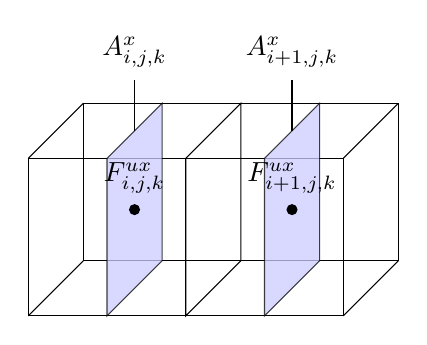
\begin{tikzpicture}
    \draw (0,0) rectangle (4,2);
    \draw (0.7,0.7) rectangle (4.7,2.7);
  
    \draw (0,0) -- (0.7,0.7);
    \draw (4,0) -- (4.7,0.7);
    \draw (0,2) -- (0.7,2.7);
    \draw (4,2) -- (4.7,2.7);
  
    \draw (2.0,0.0) -- (2.7,0.7) -- (2.7,2.7) -- (2.0,2.0) -- cycle;
 
    \filldraw[fill=blue!20, opacity=0.75] (1.0,0.0) -- (1.7,0.7) -- (1.7,2.7) -- (1.0,2.0) -- cycle;
    \node at (1.35,1.75) {$F^{ux}_{i,j,k}$};
  
    \filldraw[fill=blue!20, opacity=0.75] (3.0,0.0) -- (3.7,0.7) -- (3.7,2.7) -- (3.0,2.0) -- cycle;
    \node at (3.35,1.75) {$F^{ux}_{i+1,j,k}$};
  
    \fill (1.35,1.35) circle (2pt);
    \fill (3.35,1.35) circle (2pt);
  
    \draw (3.35,2.35) -- (3.35,3.0);
    \node at (3.35,3.35) {$A^{x}_{i+1,j,k}$};
    \draw (1.35,2.35) -- (1.35,3.0);
    \node at (1.35,3.35) {$A^{x}_{i,j,k}$};
  \end{tikzpicture}
  \caption{Blue area indicates $A^{x}$, and black dot indicates where $F^{ux}$ is calculated.}
\end{subfigure}
\hspace{0.03\linewidth}
\begin{subfigure}{0.3\linewidth}
  \centering
  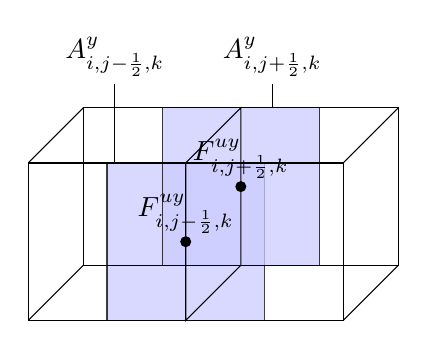
\begin{tikzpicture}
    \filldraw[fill=blue!20, opacity=0.75] (1.0,0.0) -- (3.0,0.0) -- (3.0,2.0) -- (1.0,2.0) -- cycle;
    \filldraw[fill=blue!20, opacity=0.75] (1.7,0.7) -- (3.7,0.7) -- (3.7,2.7) -- (1.7,2.7) -- cycle;

    \draw (0,0) rectangle (4,2);
    \draw (0.7,0.7) rectangle (4.7,2.7);
  
    \draw (0,0) -- (0.7,0.7);
    \draw (4,0) -- (4.7,0.7);
    \draw (0,2) -- (0.7,2.7);
    \draw (4,2) -- (4.7,2.7);
  
    \draw (2.0,0.0) -- (2.7,0.7) -- (2.7,2.7) -- (2.0,2.0) -- cycle;

    \node at (2.0,1.35) {$F^{uy}_{i,j-\frac{1}{2},k}$};
    \node at (2.7,2.05) {$F^{uy}_{i,j+\frac{1}{2},k}$};

    \fill (2.0,1.0) circle (2pt);
    \fill (2.7,1.7) circle (2pt);

    \draw (1.1,2.0) -- (1.1,3.0);
    \node at (1.1,3.35) {$A^{y}_{i,j-\frac{1}{2},k}$};
    \draw (3.1,2.7) -- (3.1,3.0);
    \node at (3.1,3.35) {$A^{y}_{i,j+\frac{1}{2},k}$};
  \end{tikzpicture}
  \caption{Blue area indicates $A^{y}$, and black dot indicates where $F^{uy}$ is calculated.}
\end{subfigure}
\caption{Placement of each terms appered in (\ref{eq:disc_diff_u}).}
\label{fig:def_point_uflux}
\end{figure}
\vspace{-10pt}

In the calculation of $\Delta v_{i,j+\frac{1}{2},k}$ and $\Delta w_{i,j,k+\frac{1}{2}}$, we assume volumes $V_{i,j+\frac{1}{2},k}$ and $V_{i,j,k+\frac{1}{2}}$, respectively, and calculate $F^{vx}, F^{vy}, F^{wx}, F^{wy}, A^x$ and $A^y$ on their faces.
Increments of $v_{i,j+\frac{1}{2},k}$ and $w_{i,j,k+\frac{1}{2}}$ are calculated in the same manner as (\ref{eq:disc_diff_u}):
\vspace{-5pt}
\begin{equation}
  \Delta v_{i,j+\frac{1}{2},k} = - \frac{
        \left( F^{vx}_{i+\frac{1}{2},j,k} A^{x}_{i+\frac{1}{2},j,k} - F^{vx}_{i-\frac{1}{2},j,k} A^{x}_{i-\frac{2}{2},j,k} \right)
      + \left( F^{vy}_{i,j+1,k} A^{y}_{i,j+1,k} - F^{vy}_{i,j,k} A^{y}_{i,j,k} \right)
                                        }{ V_{i,j+\frac{1}{2},k} } \Delta t,
  \label{eq:disc_diff_v}
\end{equation}
\vspace{-5pt}
\begin{equation}
  \Delta w_{i,j,k+\frac{1}{2}} = - \frac{
        \left( F^{wx}_{i+\frac{1}{2},j,k+\frac{1}{2}} A^{x}_{i+\frac{1}{2},j,k+\frac{1}{2}} - F^{wx}_{i-\frac{1}{2},j,k+\frac{1}{2}} A^{x}_{i-\frac{2}{2},j,k+\frac{1}{2}} \right)
      + \left( F^{wy}_{i,j+\frac{1}{2},k+\frac{1}{2}} A^{y}_{i,j+\frac{1}{2},k+\frac{1}{2}} - F^{wy}_{i,j-\frac{1}{2},k+\frac{1}{2}} A^{y}_{i,j-\frac{1}{2},k+\frac{1}{2}} \right)
                                        }{ V_{i,j,k+\frac{1}{2}} } \Delta t,
  \label{eq:disc_diff_w}
\end{equation}
Please see Figure\ref{fig:def_point_vflux} and Figure\ref{fig:def_point_wflux} for placement of each term in (\ref{eq:disc_diff_v}) and (\ref{eq:disc_diff_w}), respectively.
Similarly, volume-weighed total $v$ and $w$ are conserved through the calculation.
\vspace{-5pt}
\begin{equation}
  \Delta \left( \sum_{i,j,k} V_{i,j+\frac{1}{2},k} v_{i,j+\frac{1}{2},k} \right) = \sum_{i,j,k} V_{i,j+\frac{1}{2},k} \Delta v_{i,j+\frac{1}{2},k} = 0
\end{equation}
\vspace{-5pt}
\begin{equation}
  \Delta \left( \sum_{i,j,k} V_{i,j,k+\frac{1}{2}} w_{i,j,k+\frac{1}{2}} \right) = \sum_{i,j,k} V_{i,j,k+\frac{1}{2}} \Delta w_{i,j,k+\frac{1}{2}} = 0
\end{equation}

\begin{figure}[h]
\vspace{-15pt}
\centering
\begin{subfigure}{0.3\linewidth}
  \centering
  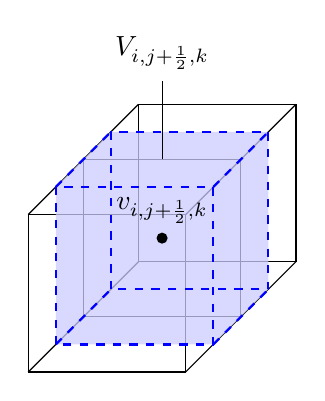
\begin{tikzpicture}
    \draw (0,0) rectangle (2,2);
    \draw (0.7,0.7) rectangle (2.7,2.7);
    \draw (1.4,1.4) rectangle (3.4,3.4);
  
    \draw (0,0) -- (1.4,1.4);
    \draw (2,0) -- (3.4,1.4);
    \draw (0,2) -- (1.4,3.4);
    \draw (2,2) -- (3.4,3.4);
   
    \filldraw[fill=blue!20, draw=none, opacity=0.75] (0.35,0.35) -- (2.35,0.35) -- (3.05,1.05) -- (3.05,3.05) -- (1.05,3.05) -- (0.35,2.35) -- cycle;
    \draw[blue, thick, dashed] (0.35,0.35) rectangle (2.35,2.35);
    \draw[blue, thick, dashed] (1.05,1.05) rectangle (3.05,3.05);
    \draw[blue, thick, dashed] (0.35,0.35) -- (1.05,1.05);
    \draw[blue, thick, dashed] (2.35,0.35) -- (3.05,1.05);
    \draw[blue, thick, dashed] (0.35,2.35) -- (1.05,3.05);
    \draw[blue, thick, dashed] (2.35,2.35) -- (3.05,3.05);
    \fill (1.7,1.7) circle (2pt);
    \node at (1.7,2.05) {$v_{i,j+\frac{1}{2},k}$};
    \draw (1.7,2.7) -- (1.7,3.7);
    \node at (1.7,4.05) {$V_{i,j+\frac{1}{2},k}$};
  \end{tikzpicture}
  \caption{Blue cube indicates $V_{i,j+\frac{1}{2},k}$, and black dot indicates where $v_{i,j+\frac{1}{2},k}$ is located.}
\end{subfigure}
\hspace{0.03\linewidth}
\begin{subfigure}{0.3\linewidth}
  \centering
  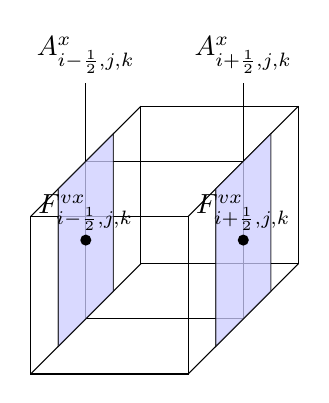
\begin{tikzpicture}
    \draw (0,0) rectangle (2,2);
    \draw (0.7,0.7) rectangle (2.7,2.7);
    \draw (1.4,1.4) rectangle (3.4,3.4);
  
    \draw (0,0) -- (1.4,1.4);
    \draw (2,0) -- (3.4,1.4);
    \draw (0,2) -- (1.4,3.4);
    \draw (2,2) -- (3.4,3.4);
 
    \filldraw[fill=blue!20, opacity=0.75] (0.35,0.35) -- (1.05,1.05) -- (1.05,3.05) -- (0.35,2.35) -- cycle;
    \node at (0.7,2.05) {$F^{vx}_{i-\frac{1}{2},j,k}$};
  
    \filldraw[fill=blue!20, opacity=0.75] (2.35,0.35) -- (3.05,1.05) -- (3.05,3.05) -- (2.35,2.35) -- cycle;
    \node at (2.7,2.05) {$F^{vx}_{i+\frac{1}{2},j,k}$};
  
    \fill (0.7,1.7) circle (2pt);
    \fill (2.7,1.7) circle (2pt);
  
    \draw (0.7,2.7) -- (0.7,3.7);
    \node at (0.7,4.05) {$A^{x}_{i-\frac{1}{2},j,k}$};
    \draw (2.7,2.7) -- (2.7,3.7);
    \node at (2.7,4.05) {$A^{x}_{i+\frac{1}{2},j,k}$};
  \end{tikzpicture}
  \caption{Blue area indicates $A^{x}$, and black dot indicates where $F^{vx}$ is calculated.}
\end{subfigure}
\hspace{0.03\linewidth}
\begin{subfigure}{0.3\linewidth}
  \centering
  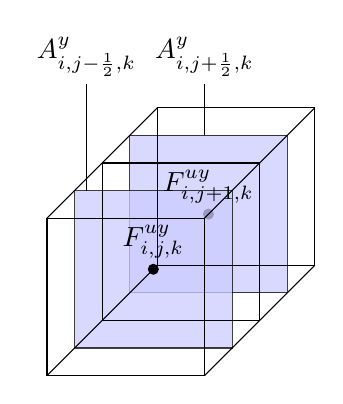
\begin{tikzpicture}
    \filldraw[fill=blue!20, opacity=0.75] (1.05,1.05) -- (3.05,1.05) -- (3.05,3.05) -- (1.05,3.05) -- cycle;
    \fill (2.05,2.05) circle (2pt);
    \draw (2.0,3.05) -- (2.0,3.7);
    \node at (2.0,4.05) {$A^{y}_{i,j+\frac{1}{2},k}$};

    \filldraw[fill=blue!20, opacity=0.75] (0.35,0.35) -- (2.35,0.35) -- (2.35,2.35) -- (0.35,2.35) -- cycle;

    \draw (0,0) rectangle (2,2);
    \draw (0.7,0.7) rectangle (2.7,2.7);
    \draw (1.4,1.4) rectangle (3.4,3.4);
  
    \draw (0,0) -- (1.4,1.4);
    \draw (2,0) -- (3.4,1.4);
    \draw (0,2) -- (1.4,3.4);
    \draw (2,2) -- (3.4,3.4);
 
    \node at (1.35,1.7) {$F^{uy}_{i,j,k}$};
    \node at (2.05,2.4) {$F^{uy}_{i,j+1,k}$};

    \fill (1.35,1.35) circle (2pt);

    \draw (0.5,2.35) -- (0.5,3.7);
    \node at (0.5,4.05) {$A^{y}_{i,j-\frac{1}{2},k}$};
  \end{tikzpicture}
  \caption{Blue area indicates $A^{y}$, and black dot indicates where $F^{uy}$ is calculated.}
\end{subfigure}
\caption{Placement of each terms appered in (\ref{eq:disc_diff_v}).}
\label{fig:def_point_vflux}
\end{figure}

\begin{figure}[h]
\vspace{-20pt}
\centering
\begin{subfigure}{0.3\linewidth}
  \centering
  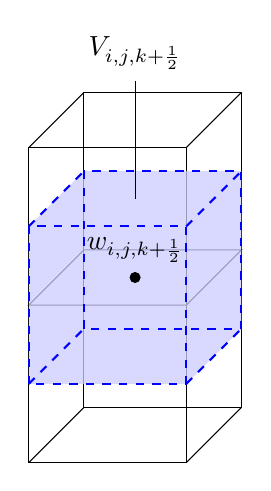
\begin{tikzpicture}
    \draw (0,0) rectangle (2,4);
    \draw (0.7,0.7) rectangle (2.7,4.7);
    \draw (0.0,2.0) -- (2.0,2.0) -- (2.7,2.7) -- (0.7,2.7) -- cycle;
    \draw (0,0) -- (0.7,0.7);
    \draw (2,0) -- (2.7,0.7);
    \draw (0,4) -- (0.7,4.7);
    \draw (2,4) -- (2.7,4.7);
   
    \filldraw[fill=blue!20, draw=none, opacity=0.75] (0.0,1.0) -- (2.0,1.0) -- (2.7,1.7) -- (2.7,3.7) -- (0.7,3.7) -- (0.0,3.0) -- cycle;
    \draw[blue, thick, dashed] (0.0,1.0) rectangle (2.0,3.0);
    \draw[blue, thick, dashed] (0.7,1.7) rectangle (2.7,3.7);
    \draw[blue, thick, dashed] (0.0,1.0) -- (0.7,1.7);
    \draw[blue, thick, dashed] (2.0,1.0) -- (2.7,1.7);
    \draw[blue, thick, dashed] (0.0,3.0) -- (0.7,3.7);
    \draw[blue, thick, dashed] (2.0,3.0) -- (2.7,3.7);
    \fill (1.35,2.35) circle (2pt);
    \node at (1.35,2.7) {$w_{i,j,k+\frac{1}{2}}$};
    \draw (1.35,3.35) -- (1.35,4.85);
    \node at (1.35,5.2) {$V_{i,j,k+\frac{1}{2}}$};
  \end{tikzpicture}
  \caption{Blue cube indicates $V_{i,j,k+\frac{1}{2}}$, and black dot indicates where $w_{i,j,k+\frac{1}{2}}$ is located.}
\end{subfigure}
\hspace{0.03\linewidth}
\begin{subfigure}{0.3\linewidth}
  \centering
  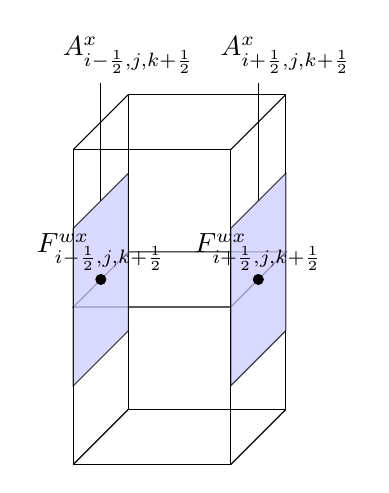
\begin{tikzpicture}
    \draw (0,0) rectangle (2,4);
    \draw (0.7,0.7) rectangle (2.7,4.7);
    \draw (0.0,2.0) -- (2.0,2.0) -- (2.7,2.7) -- (0.7,2.7) -- cycle;
    \draw (0,0) -- (0.7,0.7);
    \draw (2,0) -- (2.7,0.7);
    \draw (0,4) -- (0.7,4.7);
    \draw (2,4) -- (2.7,4.7);

    \filldraw[fill=blue!20, opacity=0.75] (0.0,1.0) -- (0.7,1.7) -- (0.7,3.7) -- (0.0,3.0) -- cycle;
    \node at (0.35,2.7) {$F^{wx}_{i-\frac{1}{2},j,k+\frac{1}{2}}$};
  
    \filldraw[fill=blue!20, opacity=0.75] (2.0,1.0) -- (2.7,1.7) -- (2.7,3.7) -- (2.0,3.0) -- cycle;
    \node at (2.35,2.7) {$F^{wx}_{i+\frac{1}{2},j,k+\frac{1}{2}}$};
  
    \fill (0.35,2.35) circle (2pt);
    \fill (2.35,2.35) circle (2pt);
  
    \draw (0.35,3.35) -- (0.35,4.85);
    \node at (0.7,5.2) {$A^{x}_{i-\frac{1}{2},j,k+\frac{1}{2}}$};
    \draw (2.35,3.35) -- (2.35,4.85);
    \node at (2.7,5.2) {$A^{x}_{i+\frac{1}{2},j,k+\frac{1}{2}}$};
  \end{tikzpicture}
  \caption{Blue area indicates $A^{x}$, and black dot indicates where $F^{wx}$ is calculated.}
\end{subfigure}
\hspace{0.03\linewidth}
\begin{subfigure}{0.3\linewidth}
  \centering
  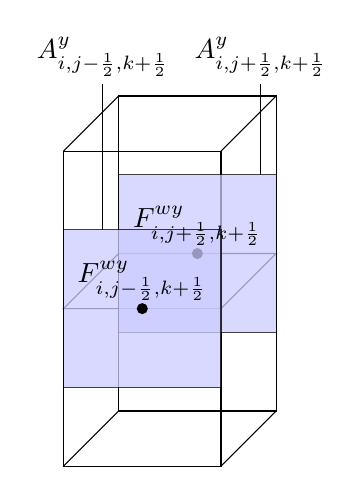
\begin{tikzpicture}
    \draw (0,0) rectangle (2,4);
    \draw (0.7,0.7) rectangle (2.7,4.7);
    \draw (0.0,2.0) -- (2.0,2.0) -- (2.7,2.7) -- (0.7,2.7) -- cycle;
    \draw (0,0) -- (0.7,0.7);
    \draw (2,0) -- (2.7,0.7);
    \draw (0,4) -- (0.7,4.7);
    \draw (2,4) -- (2.7,4.7);
 
    \filldraw[fill=blue!20, opacity=0.75] (0.7,1.7) -- (2.7,1.7) -- (2.7,3.7) -- (0.7,3.7) -- cycle;
    \fill (1.7,2.7) circle (2pt);

    \filldraw[fill=blue!20, opacity=0.75] (0.0,1.0) -- (2.0,1.0) -- (2.0,3.0) -- (0.0,3.0) -- cycle;
    \node at (1.0,2.35) {$F^{wy}_{i,j-\frac{1}{2},k+\frac{1}{2}}$}; 
  
    \fill (1.0,2.0) circle (2pt);
    \node at (1.7,3.05) {$F^{wy}_{i,j+\frac{1}{2},k+\frac{1}{2}}$};
 
    \draw (0.5,3.0) -- (0.5,4.85);
    \node at (0.5,5.2) {$A^{y}_{i,j-\frac{1}{2},k+\frac{1}{2}}$};
    \draw (2.5,3.7) -- (2.5,4.85);
    \node at (2.5,5.2) {$A^{y}_{i,j+\frac{1}{2},k+\frac{1}{2}}$};
  \end{tikzpicture}
  \caption{Blue area indicates $A^{y}$, and black dot indicates where $F^{uy}$ is calculated.}
\end{subfigure}
\caption{Placement of each terms appered in (\ref{eq:disc_diff_w}).}
\label{fig:def_point_wflux}
\end{figure}

\section{Tensorial momentum diffusion option}

Here, we will explain the equation of tensorial diffusion equation and how to calculate it.
When tensorial stress is used, (\ref{eq:base}) will be:
\vspace{-5pt}
\begin{equation}
  \frac{\partial u_i}{\partial t} = -\frac{1}{\rho} \frac{\partial F^{u_i, x_j} }{\partial x_j} \quad\quad \left( F^{u_i, x_j} = -\rho\nu \left( \frac{\partial u_i}{\partial x_j} + \textcolor{blue}{\frac{\partial u_j}{\partial x_i}} \right) \right),
  \label{eq:base_tensor}
\end{equation}
where blue colored terms are newly added in the tensorial diffusion.
Adopting imcompressive formulation, each $F^{u_i x_j}$ is represented as:
\vspace{-5pt}
\begin{equation*}
  F^{ux} = -\textcolor{blue}{2}\nu \frac{\partial u}{\partial x},
  \quad F^{uy} = -\nu \left( \frac{\partial u}{\partial y} + \textcolor{blue}{\frac{\partial v}{\partial x}} \right), 
  \quad F^{uz} = -\nu \left( \textcolor{blue}{\frac{\partial w}{\partial x}} + \textcolor{red}{\frac{\partial u}{\partial z}} \right),
\end{equation*}
\begin{equation*}
  F^{vx} = -\nu \left( \textcolor{blue}{\frac{\partial u}{\partial y}} + \frac{\partial v}{\partial x} \right),
  \quad F^{vy} = -\textcolor{blue}{2} \nu \frac{\partial v}{\partial y}, 
  \quad F^{vz} = -\nu \left( \textcolor{red}{\frac{\partial v}{\partial z}} + \textcolor{blue}{\frac{\partial w}{\partial y}} \right),
\end{equation*}
\begin{equation*}
  F^{wx} = -\nu \left( \frac{\partial w}{\partial x} + \textcolor{blue}{\frac{\partial u}{\partial z}} \right),
  \quad F^{wy} = -\nu \left( \textcolor{blue}{\frac{\partial v}{\partial z}} + \frac{\partial w}{\partial y} \right), 
  \quad F^{uz} = -\textcolor{blue}{2} \nu \textcolor{red}{\frac{\partial w}{\partial z}}.
\end{equation*}
Ignoring red colored terms, which are calculated not in the diffusion scheme but in the boundary layer scheme, the equations for $u, v$ and $w$ will be:
\vspace{-5pt}
\begin{equation}
  \frac{\partial u}{\partial t} = -\frac{\partial F^{ux}}{\partial x} - \frac{\partial F^{uy}}{\partial y} -\frac{\partial F^{uz*}}{\partial z}
  \quad \quad \left( F^{uz*} = -\nu \frac{\partial w}{\partial x}  \right),
  \label{eq:tensu}
\end{equation}
\vspace{-5pt}
\begin{equation}
  \frac{\partial v}{\partial t} = -\frac{\partial F^{vx}}{\partial x} - \frac{\partial F^{vy}}{\partial y} -\frac{\partial F^{vz*}}{\partial z}
  \quad \quad \left( F^{vz*} = -\nu \frac{\partial w}{\partial y}  \right),
  \label{eq:tensv}
\end{equation}
\vspace{-5pt}
\begin{equation}
  \frac{\partial w}{\partial t} = -\frac{\partial F^{wx}}{\partial x} - \frac{\partial F^{wy}}{\partial y}.
  \label{eq:tensw}
\end{equation}
We can calculate the first and the second terms on the right hand side of (\ref{eq:tensu}), (\ref{eq:tensv}) and (\ref{eq:tensw}) in the same way as (\ref{eq:disc_diff_u}), (\ref{eq:disc_diff_v}) and (\ref{eq:disc_diff_w}), respectively, except for adding blue colored terms in $F^{u_i x_j}$.
In the discritization of the third terms in (\ref{eq:tensu}), (\ref{eq:tensv}), we adopt a similar way so that it still conserves volume-weighed total $u$ and $v$:
\vspace{-5pt}
\begin{equation}
  -\frac{\partial F^{uz*}}{\partial z}_{i+\frac{1}{2},j,k} =
  -\frac{ F^{uz*}_{i+\frac{1}{2},j,k+\frac{1}{2}} A^z_{i+\frac{1}{2},j,k+\frac{1}{2}} - F^{uz*}_{i+\frac{1}{2},j,k-\frac{1}{2}} A^z_{i+\frac{1}{2},j,k-\frac{1}{2}} }{ V_{i+\frac{1}{2},j,k} }
  \label{eq:disc_tens_u}
\end{equation}
\vspace{-5pt}
\begin{equation}
  -\frac{\partial F^{vz*}}{\partial z}_{i,j+\frac{1}{2},k} =
  -\frac{ F^{vz*}_{i,j+\frac{1}{2},k+\frac{1}{2}} A^z_{i,j+\frac{1}{2},k+\frac{1}{2}} - F^{vz*}_{i,j+\frac{1}{2},k-\frac{1}{2}} A^z_{i,j+\frac{1}{2},k-\frac{1}{2}} }{ V_{i,j+\frac{1}{2},k} }
  \label{eq:disc_tens_v}
\end{equation}
Please see Figure\ref{fig:def_point_zflux} for placement of each term in (\ref{eq:disc_tens_u}) and (\ref{eq:disc_tens_v}).

\begin{figure}[h]
\vspace{-10pt}
\centering
\begin{subfigure}{0.3\linewidth}
  \centering
  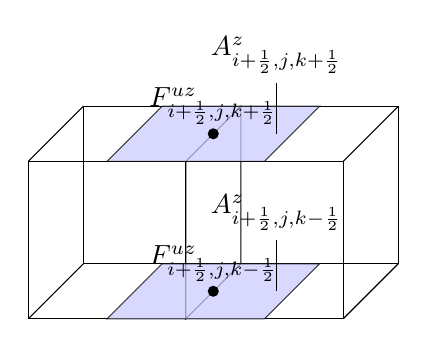
\begin{tikzpicture}
    \draw (0,0) rectangle (4,2);
    \draw (0.7,0.7) rectangle (4.7,2.7);
  
    \draw (0,0) -- (0.7,0.7);
    \draw (4,0) -- (4.7,0.7);
    \draw (0,2) -- (0.7,2.7);
    \draw (4,2) -- (4.7,2.7);
  
    \draw (2.0,0.0) -- (2.7,0.7) -- (2.7,2.7) -- (2.0,2.0) -- cycle;
 
    \filldraw[fill=blue!20, opacity=0.75] (1.0,0.0) -- (3.0,0.0) -- (3.7,0.7) -- (1.7,0.7) -- cycle;
    \node at (2.35,0.7) {$F^{uz}_{i+\frac{1}{2},j,k-\frac{1}{2}}$};
  
    \filldraw[fill=blue!20, opacity=0.75] (1.0,2.0) -- (3.0,2.0) -- (3.7,2.7) -- (1.7,2.7) -- cycle;
    \node at (2.35,2.7) {$F^{uz}_{i+\frac{1}{2},j,k+\frac{1}{2}}$};
  
    \fill (2.35,0.35) circle (2pt);
    \fill (2.35,2.35) circle (2pt);
  
    \draw (3.15,2.35) -- (3.15,3.0);
    \node at (3.15,3.35) {$A^{z}_{i+\frac{1}{2},j,k+\frac{1}{2}}$};
    \draw (3.15,0.35) -- (3.15,1.0);
    \node at (3.15,1.35) {$A^{z}_{i+\frac{1}{2},j,k-\frac{1}{2}}$};
  \end{tikzpicture}
  \caption{Blue area indicates $A^z$, and black dot indicates where $F^{uz}$ is calculated.}
\end{subfigure}
\hspace{0.03\linewidth}
\begin{subfigure}{0.3\linewidth}
  \centering
  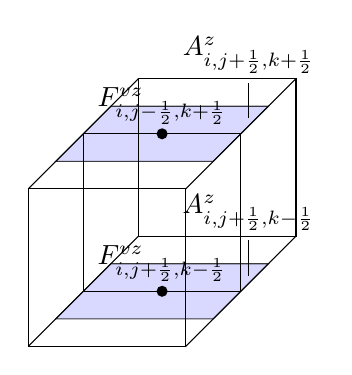
\begin{tikzpicture}
    \filldraw[fill=blue!20, opacity=0.75] (0.35,0.35) -- (1.05,1.05) -- (3.05,1.05) -- (2.35,0.35) -- cycle;
  
    \filldraw[fill=blue!20, opacity=0.75] (0.35,2.35) -- (1.05,3.05) -- (3.05,3.05) -- (2.35,2.35) -- cycle;

    \draw (0,0) rectangle (2,2);
    \draw (0.7,0.7) rectangle (2.7,2.7);
    \draw (1.4,1.4) rectangle (3.4,3.4);
  
    \draw (0,0) -- (1.4,1.4);
    \draw (2,0) -- (3.4,1.4);
    \draw (0,2) -- (1.4,3.4);
    \draw (2,2) -- (3.4,3.4);
 
 
    \fill (1.7,0.7) circle (2pt);
    \node at (1.7,1.05) {$F^{vz}_{i,j+\frac{1}{2},k-\frac{1}{2}}$};
    \fill (1.7,2.7) circle (2pt); 
    \node at (1.7,3.05) {$F^{vz}_{i,j-\frac{1}{2},k+\frac{1}{2}}$}; 

    \draw (2.8,2.9) -- (2.8,3.35);
    \node at (2.8,3.7) {$A^{z}_{i,j+\frac{1}{2},k+\frac{1}{2}}$};
    \draw (2.8,0.9) -- (2.8,1.35);
    \node at (2.8,1.7) {$A^{z}_{i,j+\frac{1}{2},k-\frac{1}{2}}$};
  \end{tikzpicture}
  \caption{Blue area indicates $A^{z}$, and black dot indicates where $F^{vz}$ is calculated.}
\end{subfigure}
\caption{Placement of each terms appered in (\ref{eq:disc_tens_u}) and (\ref{eq:disc_tens_v}).}
\label{fig:def_point_zflux}
\end{figure}

\section{Usage of function space}

In the LFRic's source code, we use $\mathbb{W}_3$ function spaces for variables placed at the center of the cell, while we use $\mathbb{W}_1$ or shifted $\mathbb{W}^H_2$ function space for variables placed on the edges of the cell.
Each degree of freedom (dof) in $\mathbb{W}_1$ and shifted $\mathbb{W}_2^H$ function space is placed as shown in Figure\ref{fig:dof}.
Function spaces used for each $F^{u_i x_j}$ is listed in table\ref{tab:def_pos}.
As shown in table\ref{tab:def_pos}, we sometimes treat 2 variables together in a single variable (e.g. we treat $F^{uy}$ and $F^{uz*}$ in a single variable uflux\_w1).


\begin{table}[h]
\centering
\begin{tabular}{|c|c|c|c|}
 \hline
 Notation in this document & Placement        & Variable name in the source code & function space \\
 \hline\hline
 $F^{ux}$ & $(i,j,k)$                         & uflux\_w3                        & $\mathbb{W}_3$                           \\ \hline
 $F^{uy}$ & $(i+\frac{1}{2},j+\frac{1}{2},k)$ & \multirow{2}{*}{uflux\_w1}       & \multirow{2}{*}{$\mathbb{W}_1$}          \\ \cline{1-2}
 $F^{uz*}$& $(i+\frac{1}{2},j,k+\frac{1}{2})$ &                                  &                                \\ \hline
 $F^{vy}$ & $(i,j,k)$                         & vflux\_w3                        & $\mathbb{W}_3$                           \\ \hline
 $F^{vx}$ & $(i+\frac{1}{2},j+\frac{1}{2},k)$ & \multirow{2}{*}{vflux\_w1}       & \multirow{2}{*}{$\mathbb{W}_1$}          \\ \cline{1-2}
 $F^{vz*}$& $(i,j+\frac{1}{2},k+\frac{1}{2})$ &                                  &                                \\ \hline
 $F^{wx}$ & $(i+\frac{1}{2},j,k+\frac{1}{2})$ & \multirow{2}{*}{wflux\_sh\_w2h}  & \multirow{2}{*}{shifted $\mathbb{W}_2^H$} \\ \cline{1-2}
 $F^{wy}$ & $(i,j+\frac{1}{2},k+\frac{1}{2})$ &                                  &                                \\ \hline
\end{tabular}
\caption{Placement and function space for each variable.}
\label{tab:def_pos}
\end{table}

\begin{figure}[h]
\centering
\begin{subfigure}{0.3\linewidth}
  \centering
  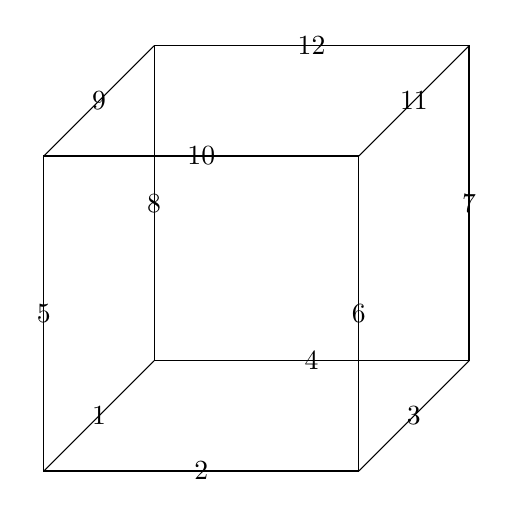
\begin{tikzpicture}
    \draw (0,0) rectangle (4,4);
    \draw (1.4,1.4) rectangle (5.4,5.4); 
    \draw (0,0) -- (1.4,1.4);
    \draw (0,4) -- (1.4,5.4);
    \draw (4,0) -- (5.4,1.4);
    \draw (4,4) -- (5.4,5.4);
    \node at (0.7,0.7) {1};
    \node at (2.0,0.0) {2};
    \node at (4.7,0.7) {3};
    \node at (3.4,1.4) {4};
    \node at (0.0,2.0) {5};
    \node at (4.0,2.0) {6};
    \node at (5.4,3.4) {7};
    \node at (1.4,3.4) {8};
    \node at (0.7,4.7) {9};
    \node at (2.0,4.0) {10};
    \node at (4.7,4.7) {11};
    \node at (3.4,5.4) {12};
  \end{tikzpicture}
  \caption{placement of each dof in $\mathbb{W}_1$ space}
  \label{fig:dof_w1}
\end{subfigure}
\hspace{15pt}
\begin{subfigure}{0.3\linewidth}
  \centering
  \begin{tikzpicture}
    \draw (0,0) rectangle (4,4);
    \draw (1.4,1.4) rectangle (5.4,5.4); 
    \draw (0,0) -- (1.4,1.4);
    \draw (0,4) -- (1.4,5.4);
    \draw (4,0) -- (5.4,1.4);
    \draw (4,4) -- (5.4,5.4);
    \node at (0.7,0.7) {1};
    \node at (2.0,0.0) {2};
    \node at (4.7,0.7) {3};
    \node at (3.4,1.4) {4};
  \end{tikzpicture}
  \caption{placement of each dof in shifted $\mathbb{W}^{H}_2$ space}
  \label{fig:dof_sh_w2h}
\end{subfigure}
\hspace{5pt}
\begin{subfigure}{0.2\linewidth}
  \vspace{-10pt}
  \begin{tikzpicture}
    \draw[->] (-0.5,0) -- (2.0,0.0) node[right] {$x$};
    \draw[->] (0,-0.5) -- (0.0,2.0) node[right] {$z$};
    \draw[->] (-0.3,-0.3) -- (1.4,1.4) node[right] {$y$};
  \end{tikzpicture}
\end{subfigure}
\caption{placement of dof}
\label{fig:dof}
\end{figure}

\section{Point to note}

\subsection{Rigor in other coordinates}

Equations solved in this scheme holds in only cartesian coordinate, but LFRic also uses other coordinates such as cubes-sphere and rotated latitude-longitude coordinates.
Strictly speaking, metric terms such as metric tensor and Christoffel symbols must be taken into account in other coordinates.

\subsection{Non-conservation in nesting run.}

This scheme is designed to calculate increments of outer most wind as 0 in the nesting run.
This design is natural since outer most wind should be always equal as that of parent model in the nesting run.
But we have to note this rigid bonudary condition breaks conservation of volume-weighed total $u, v$ and $w$ in nesting run while they are conserved rigorously in idealised simulation using periodic lateral boundary condition.
For example, given $u_{i+\frac{1}{2},j,k}$ is located at the lateral boundary in $y$-direction as depected in Figure\ref{fig:lb}, we implicitly assume $F^{uy}_{i+\frac{1}{2},j+\frac{1}{2}}$, the lateral boundary condition of $u$, so that it satisfies:
\begin{equation}
  \Delta u_{i+\frac{1}{2},j,k} =
  -\frac{\partial F^{ux}}{\partial x}_{i+\frac{1}{2},j,k}
  -\frac{\partial F^{uy}}{\partial y}_{i+\frac{1}{2},j,k}
  -\frac{\partial F^{uz*}}{\partial z}_{i+\frac{1}{2},j,k}
  = 0,
\end{equation}
that is:
\begin{equation*}
  F^{uy}_{i+\frac{1}{2},j+\frac{1}{2},k} A^{y}_{i+\frac{1}{2},j+\frac{1}{2},k} =
      F^{uy}_{i+\frac{1}{2},j-\frac{1}{2},k} A^{y}_{i+\frac{1}{2},j-\frac{1}{2},k}
    - \left(
      F^{ux}_{i+1,j,k} A^{x}_{i+1,j,k} - F^{ux}_{i,j,k} A^{x}_{i,j,k}
      \right)
\end{equation*}
\begin{equation}
    - \left(
      F^{uz*}_{i+\frac{1}{2},j,k+\frac{1}{2}} A^{z}_{i+\frac{1}{2},j,k+\frac{1}{2}} - F^{uz*}_{i+\frac{1}{2},j,k-\frac{1}{2}} A^{z}_{i+\frac{1}{2},j,k-\frac{1}{2}}
      \right)
\end{equation}
This non-zero term resides after summing up (\ref{eq:disc_diff_u}) and changes the total volume-weighed $u$.

\begin{figure}[h]
\centering
\begin{subfigure}{0.3\linewidth}
  \centering
  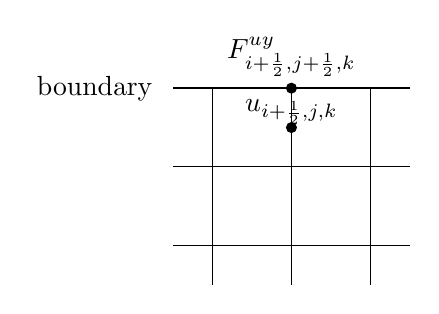
\begin{tikzpicture}
    \node at (-0.5,3.0) {boundary};
    \draw (0.5,1.0) -- (3.5,1.0);
    \draw (0.5,2.0) -- (3.5,2.0);
    \draw[thick] (0.5,3.0) -- (3.5,3.0);

    \draw (1.0,0.5) -- (1.0,3.0);
    \draw (2.0,0.5) -- (2.0,3.0);
    \draw (3.0,0.5) -- (3.0,3.0);

    \fill (2.0,3.0) circle (2pt);
    \node at (2.0,3.4) {$F^{uy}_{i+\frac{1}{2},j+\frac{1}{2},k}$};

    \fill (2.0,2.5) circle (2pt);
    \node at (2.0,2.7) {$u_{i+\frac{1}{2},j,k}$};

  \end{tikzpicture}
\hspace{5pt}
\end{subfigure}
\begin{subfigure}{0.2\linewidth}
  \vspace{-10pt}
  \begin{tikzpicture}
    \draw[->] (-0.5,0) -- (2.0,0.0) node[right] {$x$};
    \draw[->] (0,-0.5) -- (0.0,2.0) node[right] {$y$};
  \end{tikzpicture}
\end{subfigure}
\caption{Horizontal cross section close to the lateral boundary}
\label{fig:lb}
\end{figure}



\bibliographystyle{plain}
\bibliography{equation}

\end{document}


